\section{Solution}
We observe that models often over-assign the aggressor role and confuse victims or bystanders with active participants. We design a role-graph prompting strategy to make the required decomposition explicit. The role graph in Figure~\ref{fig:graph_structure.pdf} is a structured formulation of aggressive-scene understanding: each visible person is first checked for physical interaction, interacting persons are then assigned an interaction direction, and roles are derived from this direction. Persons initiating contact are treated as aggressors, persons receiving contact as victims, and non-interacting persons as bystanders. The aggressive action is inferred only after the aggressor and victim are identified, encouraging the model to bind the action to the correct participants rather than relying on saliency or generic aggression cues. In implementation, we prepend this graph-based instruction template to each multiple-choice VQA query. Detailed prompt is in Supplementary.

\begin{figure}[h!]
  \centering
    \centering
    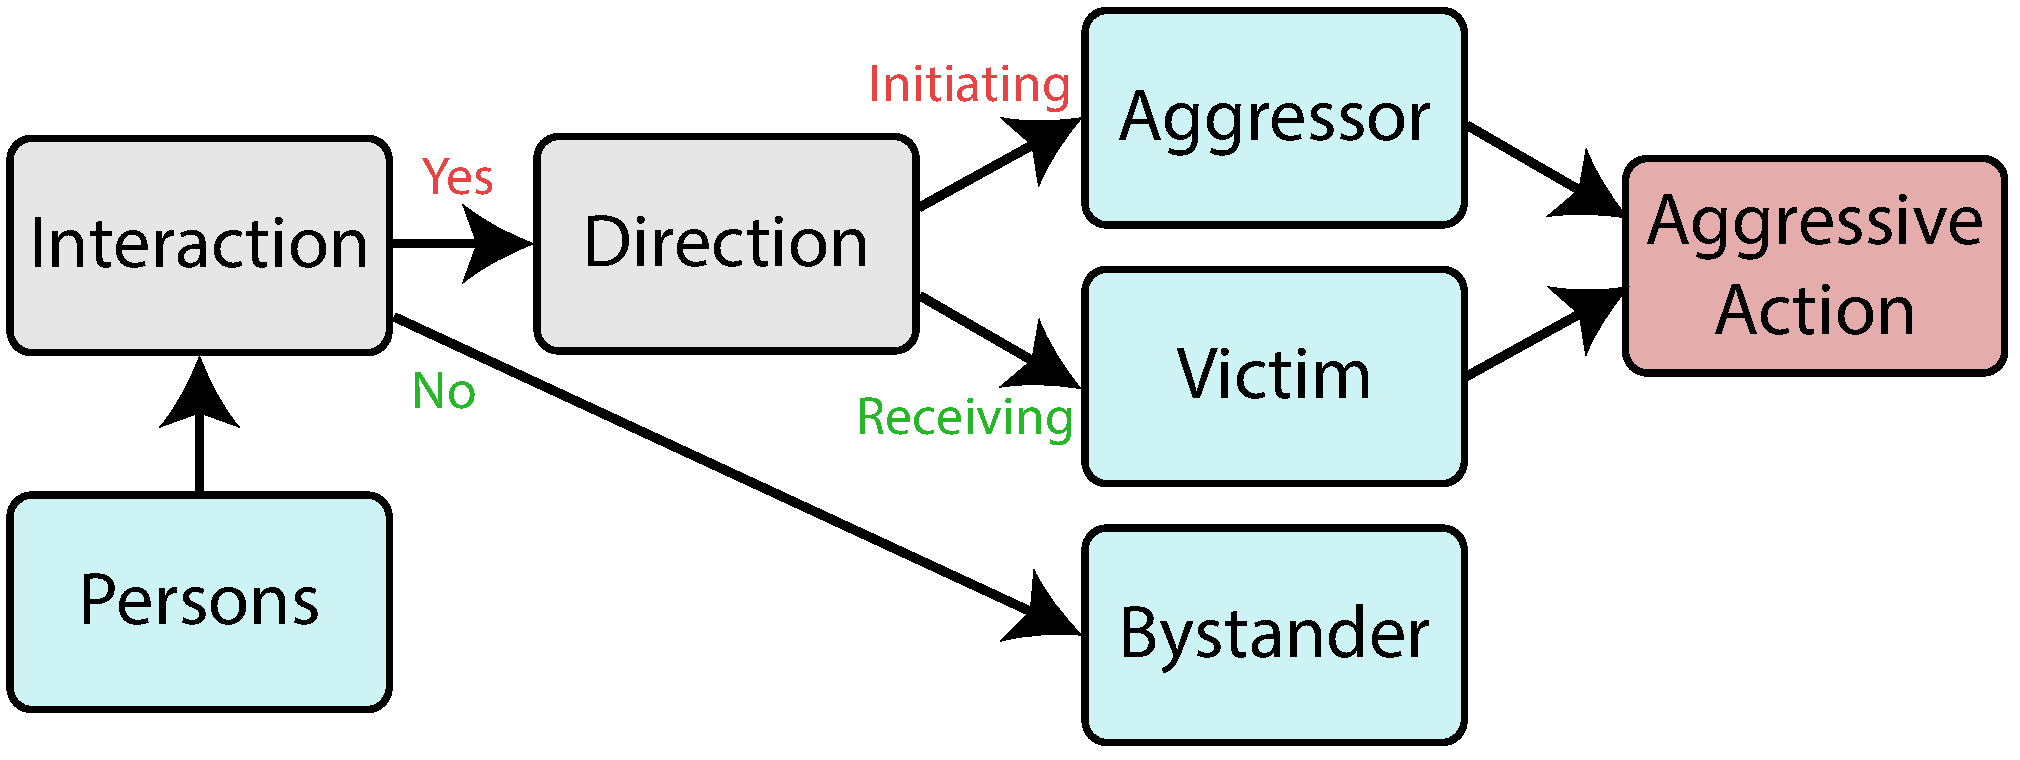
\includegraphics[width=\linewidth]{figures/graph_structure.pdf}
    
  \caption{\textbf{Graph structure?}
}

  \label{fig:graph_structure.pdf}
\end{figure}

\RA{TODO: score improvement points table}
\RA{Figure showing improvement?}